\clearpage
\section{Lösungskonzept}\label{sec:Loesungskonzept}


Zur Messung und Auswertung der Mesh-Netzwerke dient ein Testframework wie in Abbildung \ref{fig:KonzeptTestframework} ersichtlich.

\begin{figure}[H]
	\centering
	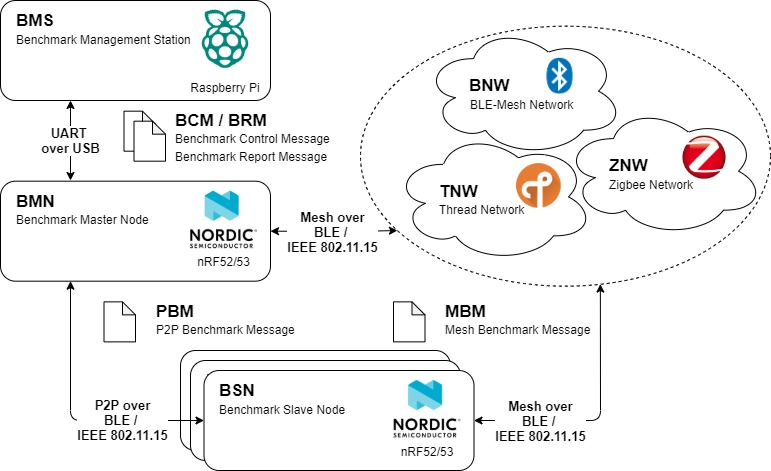
\includegraphics[width=1.0\textwidth]{Konzept_Testframework.jpg}
	\caption{Konzept Testframework}\label{fig:KonzeptTestframework}
\end{figure}


Das Testframework besteht aus folgenden physikalisch getrennten Teilsystemen:

\begin{itemize}
	\item \textbf{BMS} Benchmark Management Station \\ 
	Dient zur Verwaltung und Konfiguration des Testframeworks. Beinhaltet einen Webserver um dem Endanwender die Bedienung zu ermöglichen. Realisiert wird die BMS durch einen Raspberry Pi 4 Model B. Als Webserver wird das Python-Framework \textit{Django} eingesetzt. 
	\item \textbf{BMN} Benchmark Master Node \\ 
	Dient als Zugangspunkt der im Testframework gefahrenen Tests und lässt sich über eine Serielle Verbindung ansprechen. In der Aufgabenstellung \ref{app:Aufgabenstellung} wird von einem Master gesprochen. Realisiert wird der BMN über einen nRF52840 oder nRF5340 von \textit{Nordic}. 
	\item \textbf{BSN} Benchmark Slave Node \\ 
	Dient als Zugriffspunkt der im Testframework gefahrenen Tests und kann frei in der Testumgebung platziert werden. Daher muss die Energieversorgung über einen Akku oder Batterie erfolgen. In der Aufgabenstellung  \ref{app:Aufgabenstellung} wird von einem Slave gesprochen. Realisiert wird der BSN über einen nRF52840 oder nRF5340 von \textit{Nordic}.
\end{itemize}

Die logischen Komponenten des Testframeworks lassen sich wie folgt aufteilen:

\begin{itemize}
	\item \textbf{BCM} Benchmark Control Message \\ 
	Beschreibt Nachrichten welche zur Steuerung eines Benchmarks dienen. Dies sind zum Beispiel Konfigurations-, Start- oder Stop-Befehle. Werden vom BMS  initiiert und gelangen über eine USB-UART Verbindung zum BMN. 
	\item \textbf{BRM} Benchmark Report Message \\ 
	Beschreibt Nachrichten welche den Status oder die Ergebnisse eines Benchmarks zurückmelden. Werden vom BMN initiiert und gelangen über eine USB-UART Verbindung zum BMS.
	\item \textbf{PBM} P2P Benchmark Message \\ 
	Nachrichten welche während der Durchführung eines Benchmarks versendet werden. Dies sind zum Beispiel Ping-Anfragen zur Latenzzeitmessung. Sie ermöglichen den Datenaustausch zwischen zwei Teilnehmern auf MAC-Ebene. 
	\item \textbf{MBM} Mesh Benchmark Message \\ 
	Nachrichten welche während der Durchführung eines Benchmarks versendet werden. Dies sind zum Beispiel Ping-Anfragen zur Latenzzeitmessung. Sie ermöglichen den Datenaustausch über ein Mesh-Netzwerk auf Applikations-Ebene. 
\end{itemize}

\subsection{Punkt zu Punkt Testinfrastruktur}\label{subsec:PunktzuPunktTestinfrastruktur}

Der Punkt zu Punkt Benchmark (P2P) soll unabhängig vom Mesh-Protokoll statt finden. Damit soll es möglich sein auf MAC-Ebene BLE-Mesh (BLE) mit Thread und Zigbee (IEEE 802.11.15) zu vergleichen. Der nRF52840 sowie nRF5340 unterstützen das Arbeiten auf der MAC-Schicht. Zur Realisierung wird ein bereits bestehendes Beispiel (Radio-Example) aus der nRF Connect SDK genutzt.


\subsection{Test Mesh Netzwerke}\label{subsec:TestMeshNetzwerke}

Der Mesh-Benchmark soll die verschiedenen Mesh-Netzwerke möglichst identisch ausmessen. Dazu dient bei allen Mesh-Netzwerken die Applikations-Schicht.  

\subsubsection{Bluetooth Mesh}\label{subsubsection:Bluetooth Mesh}

Ein BLE-Mesh Netzwerk soll mit ca. 10 Knoten realisiert werden. 

\subsubsection{Thread}\label{subsubsection:Thread} 
\todo[inline]{Robin}

\subsubsection{Zigbee}\label{subsubsection:Zigbee}
\todo[inline]{Cyrill}


\subsection{Steuer und Auswertesoftware}\label{subsec:SteuerundAuswertesoftware}
\todo[inline]{Raffael}

